\documentclass{article}
\usepackage[utf8]{inputenc}

\author{Amedeo Cavallo}
\title{Reverse Engineering}

\usepackage{natbib}
\usepackage{graphicx}
\usepackage{hyperref}
\usepackage{minted}
\usepackage{tabularx}
\usepackage{tikz} 
\usepackage{pgfplots}

\usemintedstyle{fruity}  
\date{}
 
\pgfplotsset{compat=1.17}
\begin{document} 

\maketitle

\section{Introduction}

Reverse engineering is a process that examines an existing product to determine detailed information 
and specifications in order to learn how it was made and how it works. For mechanical assemblies, this typically 
involves disassembly and then analyzing, measuring and documenting the parts. Reverse engineering is not limited 
to mechanical components or assemblies. Electronic components and computer programs (software), as well as biological, 
chemical and organic matter can be reverse engineered as well. \citep{reveng}

The process of reverse engineering of software aims at restoring a higher-level representation (e.g. assembly code) 
of software in order to analyze its structure and behavior. Today, software is usually distributed in binary form 
which is, from an attacker’s perspective, substantially harder to understand than source code.
However, various techniques can be applied for analyzing binary code. \citep{codeobf}

\section{Background}

In order to figure out how to work backwards, from binary form to a higher-level representation, we need knowledge 
on the process that brought to that point. Assuming the reader to already have the knowledge on these processes,
we will revisit some key concepts, in order to have a better understanding of the reverse engineering context.

\subsection{Compilation}

The compilation is the process of converting the source code into object code. It is done with the help of the compiler. 
The compiler checks the source code for the syntactical or structural errors, and if the source code is error-free, 
it then generates the object code. \citep{compil}

Considering C programming language as reference, the C compilation process is a multistage process, and can be 
divided into four steps, i.e., Preprocessing, Compiling, Assembling, and Linking. These steps are all tipically
performed automatically.

\subsubsection{Preprocessor}

The preprocessing passes over the source code, performing these operations:
\begin{itemize}
\item Comment removal
\item Macro expansion
\item Include expansion
\item Conditional compilation (IFDEF)
\end{itemize}

\subsubsection{Compiler}

The code which is expanded by the preprocessor is passed to the compiler. Compiling converts the output of the
preprocessor into assembly instructions.

An example of what happens when you take the classic \textit{Hello World} program and compile it:
\begin{minted}[linenos, bgcolor=black, escapeinside=!!]{c}
#include <stdio.h>

int main(int argc, char ** argv) {
    printf("Hello!");
    return 0
}
\end{minted}
\begin{minted}[linenos, bgcolor=black, escapeinside=!!]{c}
.LC0:
            .string         "Hello!"
            .text
            .globl          main
            .type           main, @function
main:
.LFB0:
            .cfi_startproc
            pushq           %rbp
            .cfi_def_cfa_offset 16
            .cfi_offset     6, -16
            movq            %rsp, %rbp
            .cfi_def_cfa_register   6
            movl            $.LC0, %edi
            movl            $0, %eax 
            call            printf
            movl            $0, %eax 
            popq            %rbp 
            .cfi_def_cfa    7, 8
            ret 
            .cfi_endproc 
\end{minted}

\subsubsection{Assembler}

The assembly code is converted into object code by using an assembler. Assemblers convert the assembly code into
binary opcodes. Assuming a specific class of processors and its compatible assembly language (e.g. 
\texttt{x86} assembly language), i.e. the instruction \texttt{mov rax, 1} is represented by the binary opcode
\texttt{0x48C7C001000000}.

\subsubsection{Linker}

More is needed before the object code can be executed. Mainly, all the programs written in C use library functions. 
These library functions are pre-compiled, and the object code of these library files is stored with '.lib' (or '.a') 
extension. The main working of the linker is to combine the object code of library files with the object code of our 
program, i.e., if the printf() function is used in a program, then the linker adds its associated code in an output file. 
The result of linking is the final executable program.

\noindent\linebreak
What happens after everything has been linked is we finally have an executable output format. The output of the
compilation process can take many forms depending on the operating system:
\begin{itemize}
\item PE (Windows)
\item ELF (Linux)
\item Mach-O (OSX)
\item COFF/ECOFF
\end{itemize}
This output file is often the starting point as a reverse engineer. For the scope of this document we will
focus on the ELF format.

\subsection{ELF Format}

ELF (Executable and Linkable Format) is the object file, executable program, shared object and core file format 
for Linux and many UNIX operating systems. An ELF file contains an ELF header at the beginning of the file. 
The size of the ELF header is fixed and it contains information about the program header table and section header table. 
These values are zero if they are not present. \citep{elf}

The program header table, which is optional, tells how to create a process image. The section header table 
contains an array of Elf32 Shdr structures, which contain information about the various sections in the file. 
There can be any number of sections in the executable. Some of the common sections present in a typical binary 
are .bss, .data, .dynamic, .debug, .got, .fini., .hash, .interp, .rodata and .text. \citep{stripped}
\begin{figure}[H]
\centering
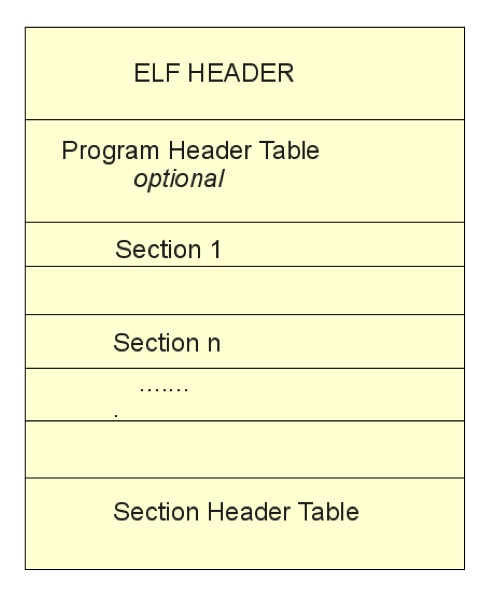
\includegraphics[width=0.4\textwidth]{img/ELF_Format.jpg}
\caption{ELF Format}
\label{fig:elf}
\end{figure}
The ELF files components extremely useful for reverse engineering are debug symbols. Symbols are used
to aid in debugging and provide context to the loader. ELF objects contain a maximum of two symbol tables:
\begin{itemize}
\item{\textbf{.symtab:}} Symbols used for debugging / labelling
\item{\textbf{.dynsym:}} Contains symbols needed for dynamic linking
\end{itemize}
The removal of these symbols (stripping) makes things more difficult to reverse engineer.

\subsection{Stripped Binary}

Stripped binaries are binaries which lack information regarding the locations, offsets, sizes and layout of functions 
as well as objects. Typically, all this information is stored in a symbol table which is generated by the compiler, 
but is removed before distribution. Although there is no performance improvement to be had by stripping a binary it 
could be done for various reasons. Commercial code is stripped to make it difficult to reverse engineer proprietary 
algorithms; system libraries are stripped to reduce the size on disk; and malware is stripped to obfuscate it and 
thus complicate analysis. The general assumption across these applications is that the absence of symbol tables 
makes analysis of binaries more difficult. \citep{stripped}

Stripped binary can be produced with the help of the compiler itself, e.g. GNU GCC compilers' -s flag, or with 
a dedicated tool like strip on Unix.

\pagebreak
\section{Binary Analysis}

The reverse engineering process is a sequence of static and dynamic analysis that slowly refine the knowledge 
about the malware sample.

\subsection{Static Analysis}

Static analysis is performed without running the software that is to be analyzed, examining code, assets and 
dependencies. It is generally thought of as a more complex approach as it usually requires in-depth knowledge 
about the platform software is run on, frameworks being used by software and, depending on the programming language 
and environment used, the language software is compiled to. 

Disassemblers interpret the raw bytes that represent the x86 and x64 assembly and display them in a human-readable 
fashion using mnemonics (e.g. translating \texttt{0xb864000000} to \texttt{mov eax, 0x40}). In case of software 
that is compiled down to bytecode using intermediate languages (such as Java or C\#) one can use decompilers
that reconstruct code that often is nearly identical to the original source-code.

\subsubsection{Disassemblers}

Disassemblers convert binary code to symbolic assembly language representations. A primary function of disassemblers 
is to visually present these assembly language representations of binary code to human analysts. To aid the analyst 
by organizing information, some disassemblers present control flow information or attempt to partitionprograms into 
functions. \citep{disass}
\begin{figure}[H]
\centering
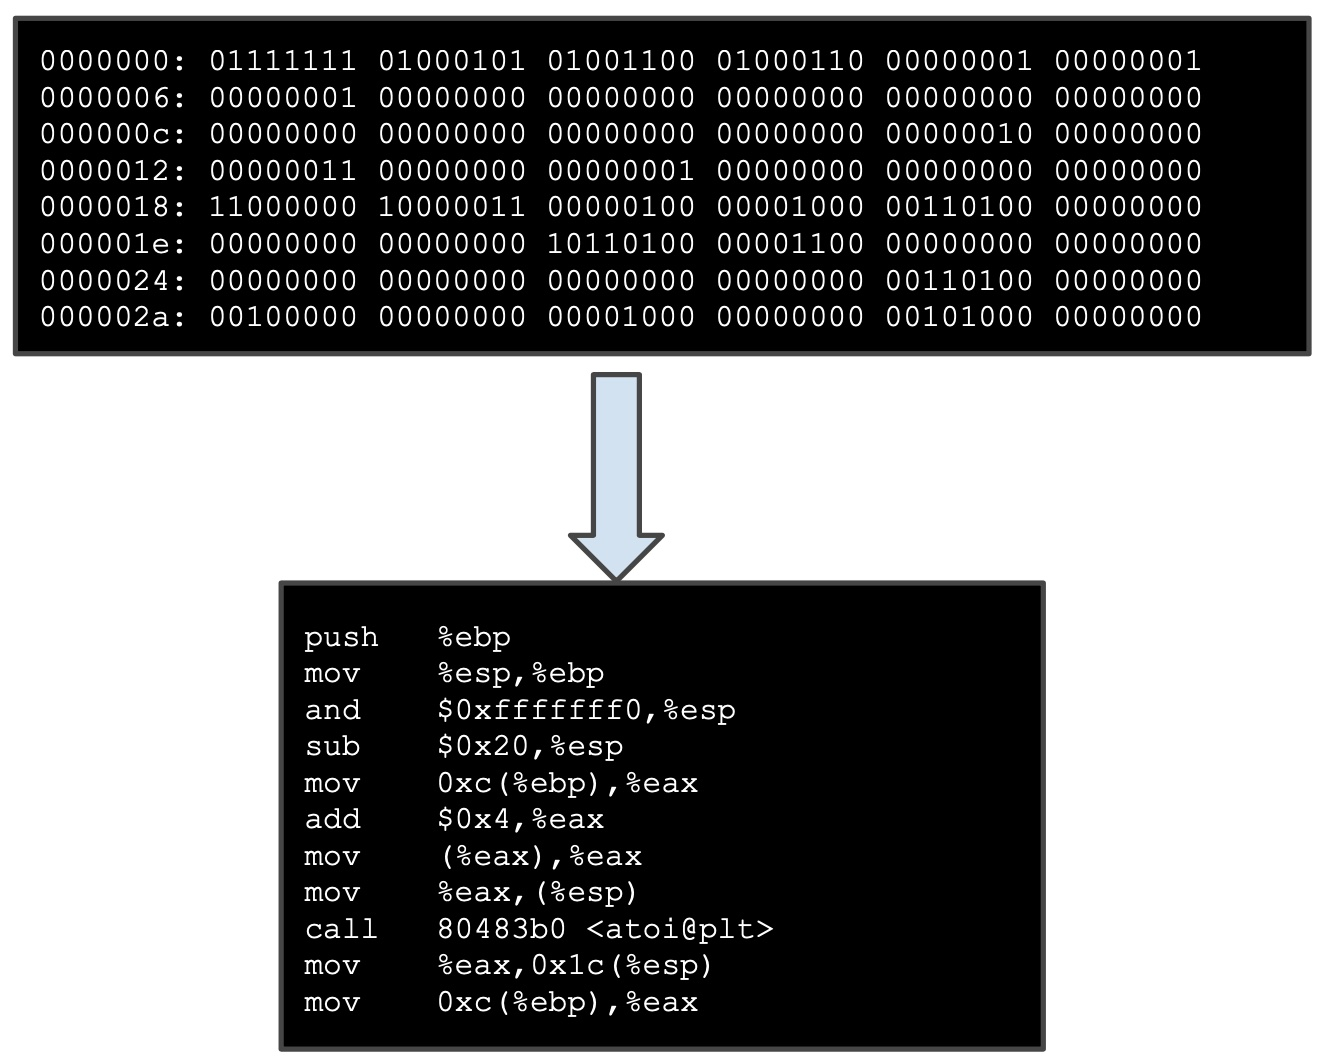
\includegraphics[width=0.7\textwidth]{img/disassembler.jpg}
\caption{Static Analysis - Disassembler}
\label{fig:disassembler}
\end{figure}
Producing correct disassembly is often challenging due variable length instruction sets, data mixed with code,
indirect control flow, and deliberate code obfuscation.

There are two basic techniques for disassembly \citep{stripped}:
\begin{itemize}
\item{\textbf{Linear Sweep:}} This is the most straightforward and simple approach to disassembly. 
Examples of such a disassembler is the GNU disassembler, \texttt{objdump}. Disassembly starts from the entry point which 
is obtained in the header of the binary (e entry field in ELF format binaries used on moat UNIX operating systems). 
Each successive instruction is disassembled from the next location, which is obtained by adding the length of the 
current instruction to the start address of the instruction. The basic disadvantage of this technique is that it 
cannot distinguish data from code. Any data embedded in the code is erroneously disassembled.
\item{\textbf{Recursive Traversal:}} Recursive traversal algorithm has some advan- tages over linear sweep since 
it takes into consideration the control flow in the binary. Thus it does not misinterpret data as code. When a 
jump instruction is decoded, the disassembler continues disassembly from the jump target instead of blindly 
disassembling the next instruction. The key problem in this approach arises in the presence of indirect control 
flow transfer. Code that is reachable only via such transfers will not be disassembled by a vanilla recursive 
disassembly algorithm.
\end{itemize}

\subsubsection{Decompiler}

Decompilers take the process a step further and actually try to reproduce the code in a high level language. 
Decompilation does have its drawbacks, because lots of data and readability constructs are lost during the original 
compilation process, and they cannot be reproduced.
\begin{figure}[H]
\centering
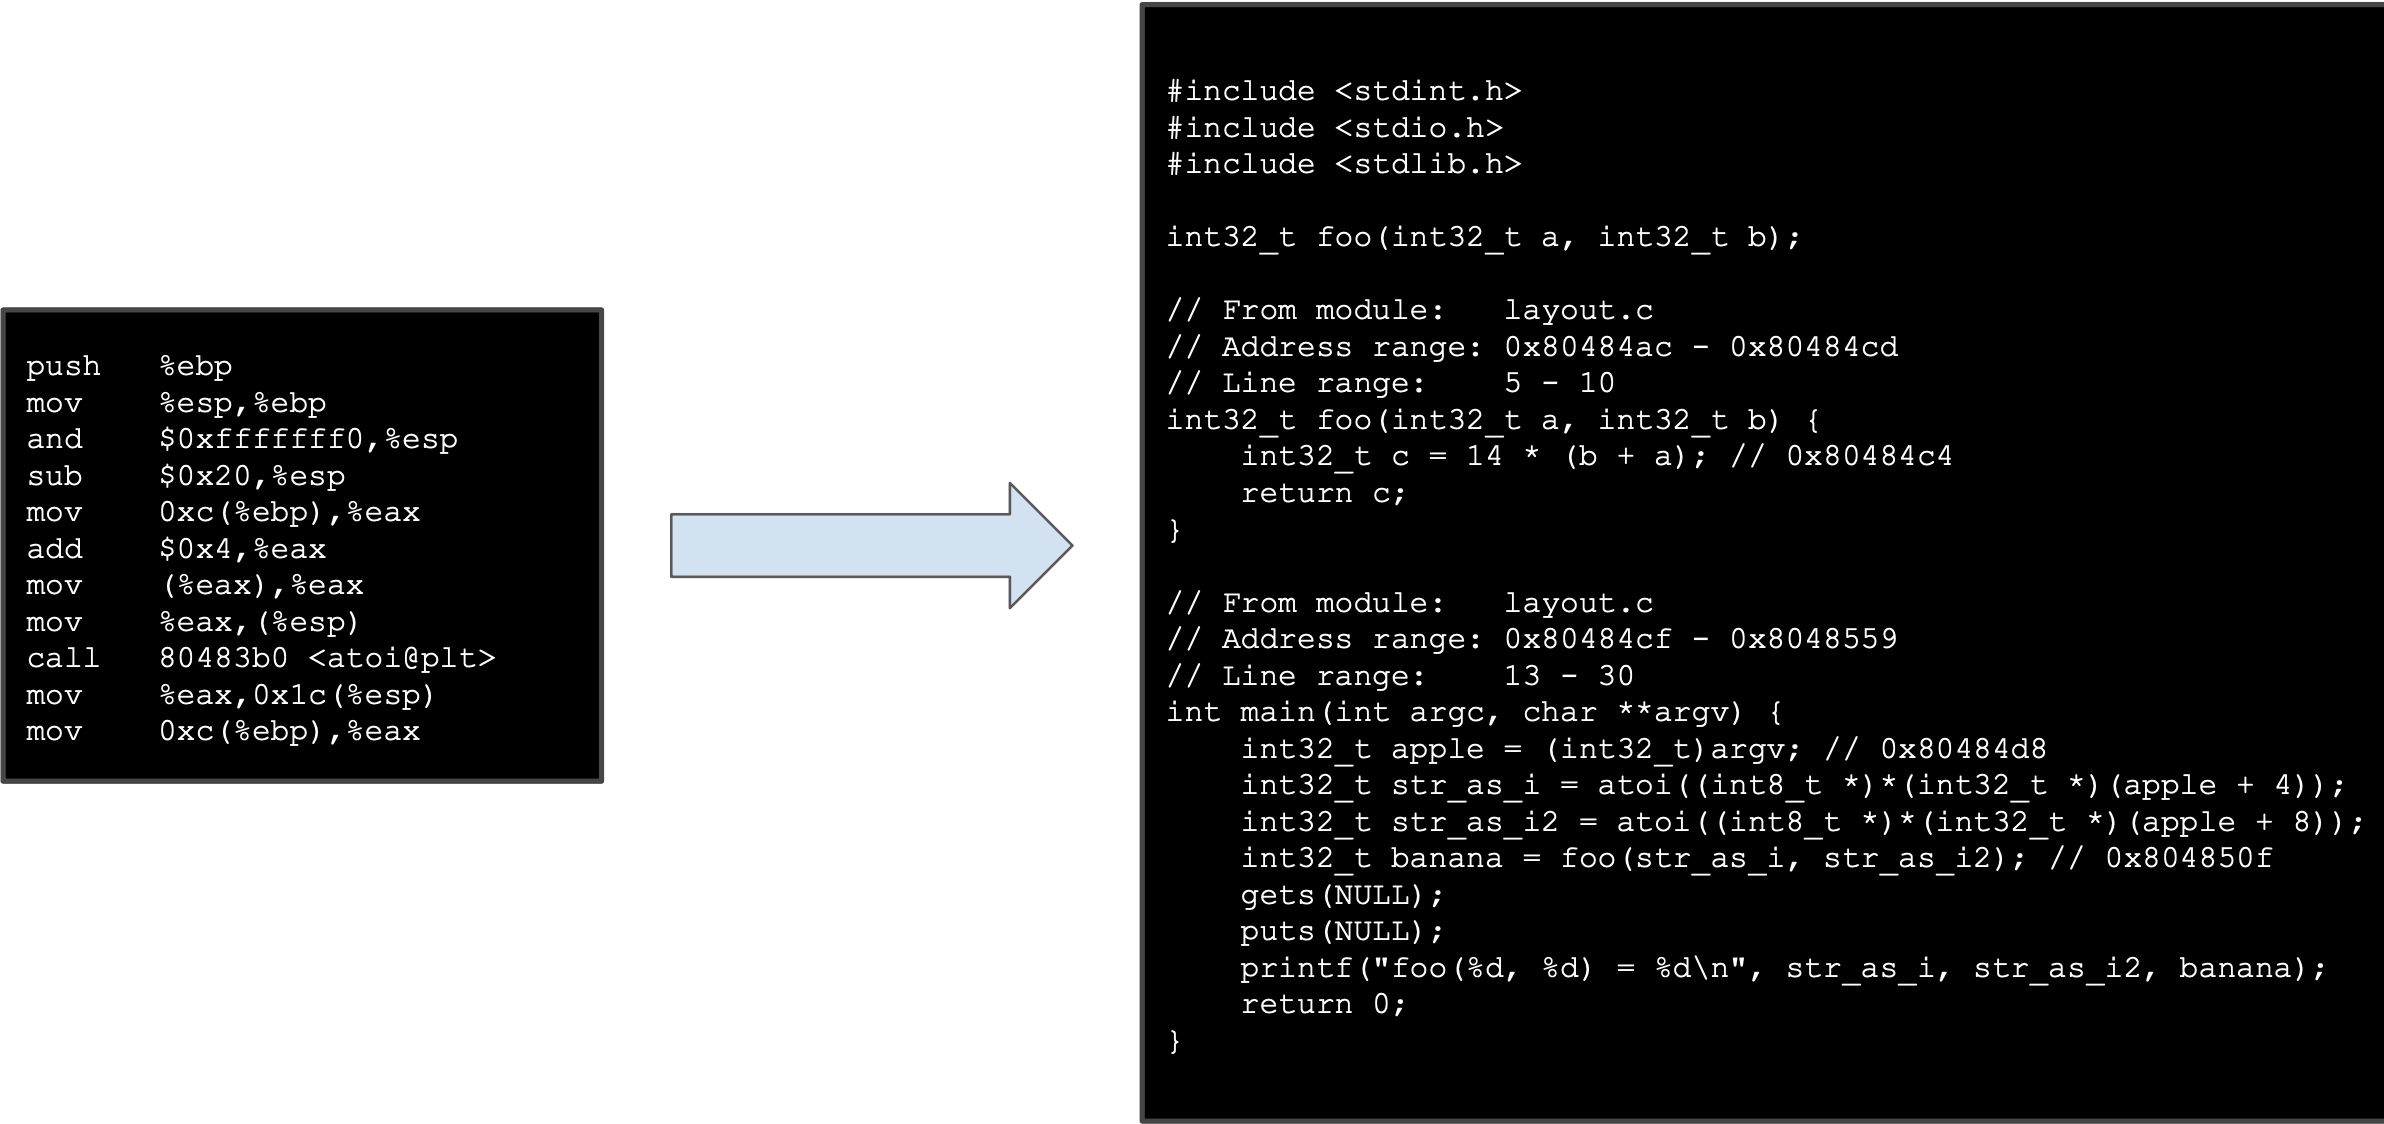
\includegraphics[width=0.9\textwidth]{img/decompiler.jpg}
\caption{Static Analysis - Decompiler}
\label{fig:decompiler}
\end{figure}

\subsubsection{Tools}

\begin{itemize}
\item objdump - Disasm
\item radare2 - Disasm
\item capstone - Programmable Disasm
\item Binary Ninja - Disasm + Primitive Decompiler
\item GHIDRA - Disasm + Decompiler
\item IDA Pro - Disasm + Decompiler (de facto standard)
\item Angr - Binary Analysis (VEX IR) + Symbolic Execution
\item rev.ng - Binary analysis with LLVM IR + Binary translationtion
\item BAP - Binary analysis with BIL IR
\end{itemize}

\subsubsection{Types}

Part of the process of reverse engineering is understanding the types in the program, creating the correct
structs and assigning the correct types to variables. Building correct types make decompilation more readable
and easy to understand.

As an example, the same decompiled function, but on the right with the correct structs assigned to the variables:
\begin{figure}[H]
\centering
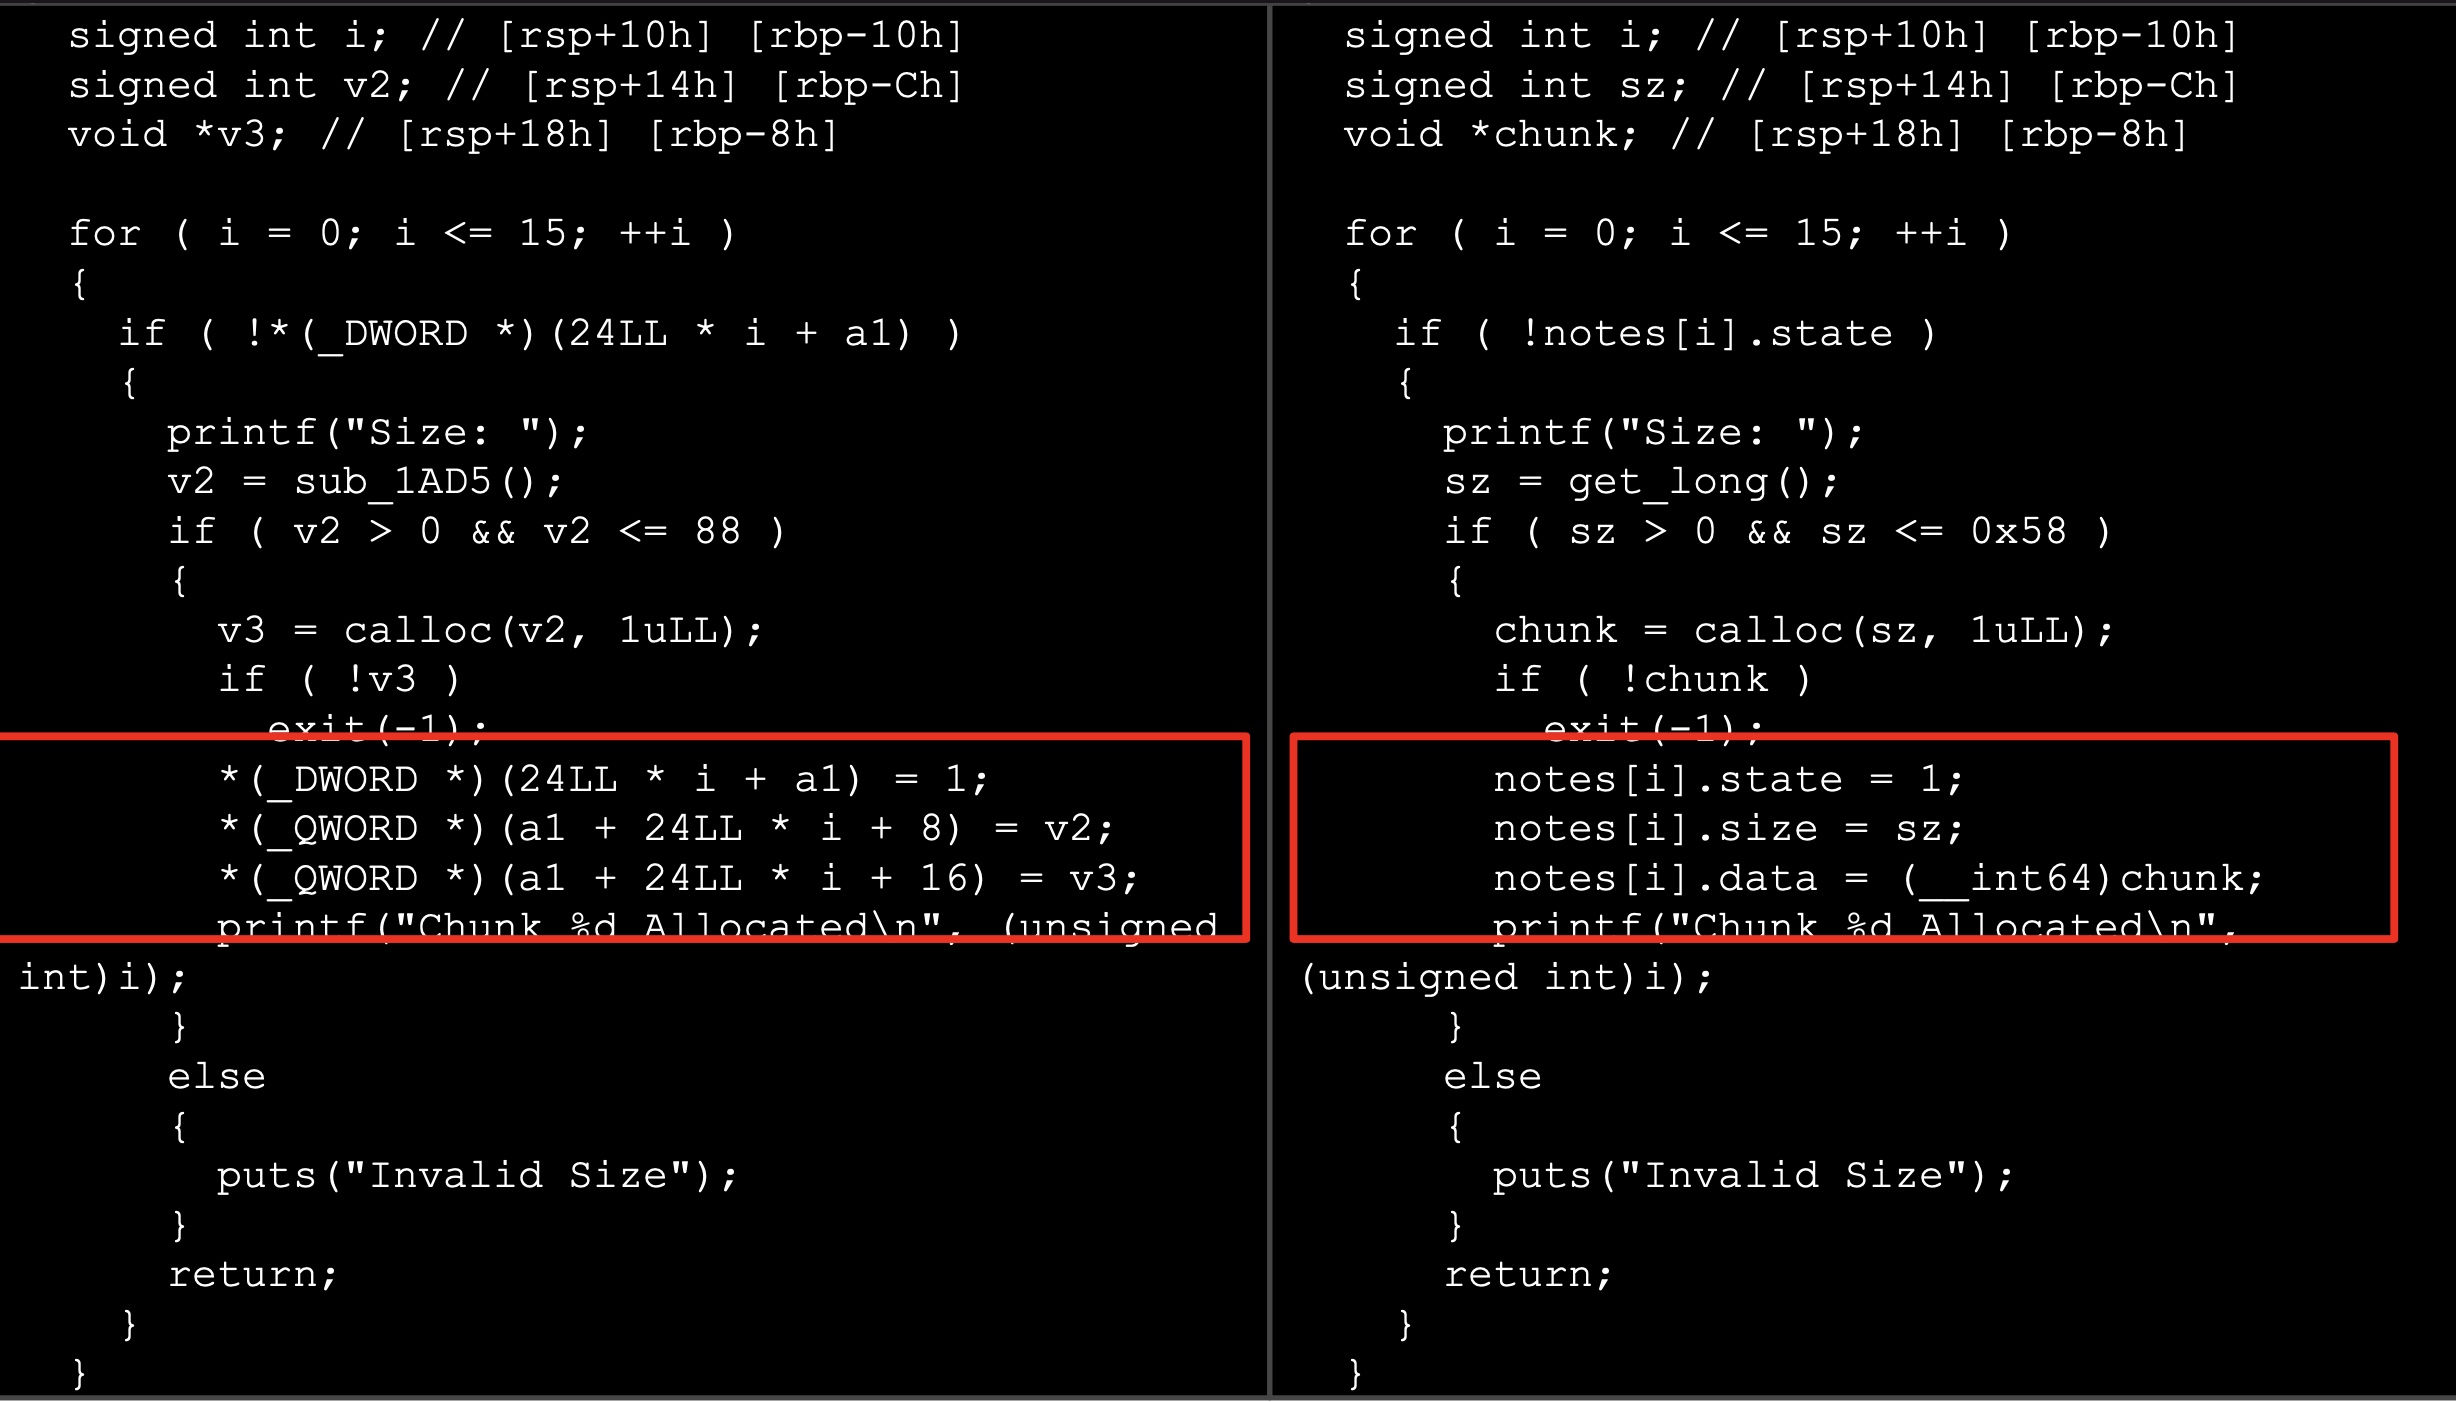
\includegraphics[width=1\textwidth]{img/struct.jpg}
\caption{Static Analysis - Struct}
\label{fig:struct}
\end{figure}

\subsection{Dynamic Analysis}

Dynamic analysis is used to observe data and behaviour at runtime. It uses some very intuitive and easy to 
understand concepts such as memory scanners and debuggers. Memory scanners allow reverse-engineers to observe 
and scan memory of running programs. They can be used to find the location of values of interest and manipulate them.
Debuggers instead, allow us to halt programs, execute instructions one at a time, examine registers and stack frames 
and trace function calls. They are especially useful to dereference pointer-chains, intercept calls to functions 
of interest and understand how data of interest is being accessed at runtime.

\subsubsection{GDB}

The GNU Debugger (GDB) is a portable debugger that runs on many Unix-like systems and works for many programming 
languages, including Ada, C, C++, Objective-C, Free Pascal, Fortran, Go, and partially others.

Standard GDB is not suitable to use for reverse engineering and exploit development, i.e. it still lacks a hexdump 
command. \texttt{pwndbg} is a GDB plug-in with a focus on features needed by low-level software developers, hardware 
hackers, reverse engineers and exploit developers. 

A small subset of usefull features are \citep{pwngdb}:
\begin{itemize}
\item{\textbf{Watch Expressions:}} You can add expressions to be watched by the context.
\item{\textbf{Disassembly:}} \texttt{pwndbg} uses Capstone Engine to display disassembled instructions, but also 
leverages its introspection into the instruction to extract memory targets and condition codes.
\item{\textbf{Heap Inspection:}} \texttt{pwndbg} enables introspection of the glibc allocator, ptmalloc2, via a 
handful of introspection functions.
\item{\textbf{Process State Inspection:}} Use the \texttt{procinfo} command in order to inspect the current process state, 
like UID, GID, Groups, SELinux context, and open file descriptors.
\item{\textbf{ROP Gadgets:}} \texttt{pwndbg} makes using ROPGadget easy with the actual addresses in the process.
\item{\textbf{Finding Leaks:}} Finding leak chains can be done using the \texttt{leakfind} command. It recurisvely 
inspects address ranges for pointers, and reports on all pointers found.
\item{\textbf{Virtual Memory Maps:}} \texttt{pwndbg} enhances the standard memory map listing, and allows easy searching.
\end{itemize}

\pagebreak
In order to exploit the full potential of \texttt{pwndbg}, knowledge of the most commonly used features of standard
GDB are required:
\begin{itemize}
\item{\textbf{Disassemble:}}
\begin{minted}[linenos, bgcolor=black, escapeinside=!!]{c}
set disassembly-flavor intet #sets syntax
disass *address #disassemble
\end{minted}
\item{\textbf{Execution:}}
\begin{minted}[linenos, bgcolor=black, escapeinside=!!]{c}
step (s) #exec nextline - enter fun
next (n) #exec nectline - jump call
finish (f) #exec til ret
continue (c) #continue execution
\end{minted}
\item{\textbf{Examine:}}
\begin{minted}[linenos, bgcolor=black, escapeinside=!!]{c}
x/numF *address #show num data of type F (bx, wx, gx, c, s)
printf “%c”, $reg #print char from register
\end{minted}
\item{\textbf{Breakpoints:}}
\begin{minted}[linenos, bgcolor=black, escapeinside=!!]{c}
b *address #set software breakp at addr
hb *address #set hardware breakp at addr
b *address if $reg==val #set conditional breakp
del br_num #remove breakpoint br_num
\end{minted}
\item{\textbf{Watchpoints:}}
\begin{minted}[linenos, bgcolor=black, escapeinside=!!]{c}
w *address #set watch for write at addr
rw *address #set watch for read at addr
\end{minted}
\item{\textbf{Registers:}}
\begin{minted}[linenos, bgcolor=black, escapeinside=!!]{c}
set $reg = val #set register to a certain value
\end{minted}
\item{\textbf{Automate:}}
\begin{minted}[linenos, bgcolor=black, escapeinside=!!]{c}
#create command that are runned after a breakp
commands br_num
    command_list
end
\end{minted}
\end{itemize}

\section{Adversarial Contest}

In some applications there is a need for software developers to protect their software against reverse engineering. 
The protection of intellectual property (e.g. proprietary algorithms) contained in software, confidentiality reasons, 
and copy protection mechanisms are the most important examples. Another important aspect are cryptographic algorithms 
such as AES. \citep{codeobf} The most common example instead are malwares, where code obfuscation and analysis
mitigations are applied in order to not be identified as that.

\subsection{Static Analysis Mitigations}

\begin{itemize}
\item{\textbf{Complex CFG:}} Create a complex control flow graph (CFG). Not aligned jumps to break the disassembler, 
modifying the compiler to add those instructions everywhere in the program. This usually will affect 
performance, so people tend to use this on code that doesn’t need performance very much. Another example is adding 
dead code, code that is never executed.
\item{\textbf{Packing:}} A technique to hide the real code of a program through one or more layers of compression / 
encryption. At run-time the unpacking routine restores the original code in memory and then executes it.
\item{\textbf{Header Corruption:}} Most of analysis tools relies on what is written in the header of the binary,
i.e. GDB and Ghidra read the header searching for symbols in the program. Messing with the header will affect the
output of the decompilation process.
\end{itemize}

\subsection{Dynamic Analysis Mitigations}

\begin{itemize}
\item{\textbf{Debugging Only Once:}} GDB is able to debug programs calling the syscall \texttt{ptrace} with the PID of
the program as a parameter. The key point is that only one instance of \texttt{ptrace} can be called simultaneously. 
The program can debug itself, autonomously calling \texttt{ptrace}, resulting in GDB not being able to attach to 
the process.
\item{\textbf{Check for Debugger:}} \texttt{0xcc} is the byte used by debuggers for breakpoints, so continuously
spamming \texttt{0xcc} to the program to execute makes debugging harder.
\item{\textbf{Divert Execution:}} Add really complicated control flows, i.e. using multithreades programs or 
sending signals to trigger functions instead of calling it.
\end{itemize}

\pagebreak
% \section{Walkthrough}    

\bibliographystyle{unsrt}
\bibliography{references}
\end{document}
